\chapter{Einführung in die Problematik}
Diese Masterarbeit beschreibt den potentiellen Nutzen eines grafischen Management Systems für die Gebäudeüberwachung mittels verschiedener stationärer und mobiler Sensoren. Anhand eines Beispieles soll geklärt werden welche Technologien eingesetzt werden müssten um diese Aufgabe zu lösen, und worin genau der Mehrwert eines solchen Systems gegenüber konventioneller Vermessungssoftware liegt. Die vorgeschlagenen Technologien werden zum Abschluss der Arbeit teilweise praktisch angewandt respektive umgesetzt. Dieser Prototyp soll exemplarisch demonstrieren wie solch ein System arbeiten wird. Kernfragen der Masterarbeit ist, wie kann dieses System Feldingenieuren, die im Bereich der Gebäudeüberwachung arbeiten, generell in den folgenden Bereichen unterstützen:
\begin{itemize}
\item Planung und Optimierung der allgemeinen Arbeiten im Feld
\item Datenkommunikation mit dem Büro
\item Vorabauswertung der Messwerte direkt im Feld
\end{itemize}
Die Klassische Arbeit von Vermessungsingenieuren besteht aus dem praktischen Teil der im Feld durchgeführt wird, und den anschließenden Auswertungen und der Interpretation im Büro. Durch die räumliche Trennung dieser Beiden dennoch sehr ineinander verzahnten Aufgaben entsteht oftmals eine Verzögerung in den Abläufen und erhöhtes Risiko für vermeidbare Fehler in den Arbeitsabläufen. Das System soll so konzeptioniert sein, dass es die Lücke schließt, zum Einen um die Effizienz der Arbeiten zu erhöhen, und zum Anderen um Fehler bei den Messungen oder der Datenmigration zu erkennen oder von vorn herein zu vermeiden. 

Heutzutage ist das Bearbeiten von unterschiedlichen Arbeiten an einem Ort zur gleichen Zeit keine Vision mehr. Mobile Endgeräte wie "Smartphones" oder "Tablet-Computer" vereinfachen Arbeitsabläufe, und helfen Zeit zu sparen. Bei den Arbeiten im Feld sind mobile Endgeräte bereits ständig präsent, dennoch helfen sie lediglich bei wenigen Aufgaben wie der papierlosen Bürokratie, der Email-Kommunikation mit dem Büro oder den betrachten vorheriger Messerergebnisse. Das hier konzipierte System hingegen weißt folgende drei Hauptvorteile gegenüber der aktuellen Nutzung von mobilen Endgeräte auf:
\begin{itemize}
\item Kernfunktionalität ist das Assistieren des Vermessungsingenieurs. Das heißt es soll Hilfestellung beim Verstehen der Messungen geben (zum Beispiel durch den Vergleich der aktuellen Messungen mit vergangenen Messreihen). $\rightarrow$ Das Teilen von Informationen zwischen Feld und Büro führt zu einem besseren Kenntnisstand während der Arbeiten im Feld.
\item Fehlmessungen wie sie etwa beim vertauschen von Positionen geschehen sollen vermieden werden indem die Messergebnisse direkt nach Eingabe in das System auf ihre Konsistenz hin überprüft werden.
\item Für die Aufnahmen im Feld brauchen vorherige Messreihen nicht umständlich exportiert zu werden, sondern diese können von dem Mobilen System direkt von dem gemeinsamen Daten-
\newglossaryentry{Server}
{
  name={Server},
  description={Elektronisches System mit dem über das TCP/IP kommuniziert werden kann, und das aktiv und passiv Dienste anbietet bzw. ausführt.},
  sort=Server
} \gls{Server} abgerufen werden.
\end{itemize}
Das hier konzeptionierte System ist keine Alternative für klassische Vermessungssoftware, ist es eine Ergänzung und eine Brücke von den Sensoren direkt zu dem System. Es ermöglicht die Kombination von klassischer Ingenieurvermessung mit Sensornetzwerken.

\chapter{Softwareanforderungen}
Die Konzeptions eines Systems muss den Anforderungen der Nutzer entsprechen, und darf nicht an dem bestehenden Bedürfnissen "vorbei geplant" werden. Die Anforderungen an das System ergeben sich aus technischen Anforderungen, Erwartungen potentieller Nutzer und die damit einhergehenden Beispielfunktionen des Systems. Der Aufbau des Anforderungskataloges besteht aus einer Beschreibung des Einsatzgebietes, einer Beschreibung des Systems und den daraus abzuleitenden funktionalen und nicht-funktionalen Anforderungen.

\section{Einsatzgebiet}
Um präzise beschreiben zu können was das System tun können muss, ist es notwendig vorher konkret die vorliegende Situation oder das existierende Problem zu definieren. Solche eine Definition sollte eine Beschreibung der Umgebung beinhalten in der das System eingesetzt werden soll. Nimmt man eine Modellierungssprache zur Hilfe, um die Umgebung zu beschrieben, ist es später einfacher daraus Rückschlüsse auf mögliche Probleme zu ziehen. Für ein solches Modell müssen die Fragen beantwortet werden, in welche Objekte sich die Umgebung aufgliedert, wie diese interagieren und welche Funktionalitäten diese dafür verwenden.Aber auch die teilhabenden Akteure und ihre konkreten Anforderungen an das System müssen modelliert werden. Mit Hilfe von exemplarischen Anwendungsfällen werde ich beschreiben was der tatsächliche Bedarf des Nutzers ist, und wie dieser gedeckt werden kann.

Bevor ich mit dem technischen Ausformulieren der Modellierung beginne, möchte ich kurz in die Thematik einleiten: Das System welches ich mit dieser Arbeit konzeptioniere soll Feldingenieuren helfen im Feld mit den Messungen und Daten verschiedener Sensoren zu arbeiten. Als konkretes Beispiel werde ich den Einsatz des Systems bei der Bauwerksüberwachung mithilfe eines Sensornetzwerkes beschreiben.

Die Überwachung von Bauwerken mittels eines Netzwerkes aus verschiedenen Sensoren hilft ihre Sicherheit ohne den Einsatz großer Bautechnischer Überprüfungen einschätzen zu können. Damit ist es möglich Bauwerke auch weit über ihre geplante Lebensdauer hinweg zu erhalten. Ohne den Einsatz solcher Sensor Netzwerke können die zuständigen Gutachter bei Ablauf der geplanten Lebensdauer nicht darauf vertrauen, dass das Gebäude auch weiterhin den kontinuierlichen Belastungen gewachsen ist, und somit werden entweder umfangreiche Sanierungen Nötig, oder Gebäude werde geschlossen. Die Überwachung basiert auf der Messung von Veränderungen von verschiedenen Parametern wie zum Beispiel der Position , der Temperatur oder Feuchtigkeit von Bauteile oder der Abweichungen von charakteristischen Bewegungsmustern von Bauteilen, gemessen durch Beschleunigungssensoren. Die Parameter werden sowohl punktuell  verteilt über das gesamt Bauwerk, als auch gesamtheitlich die Struktur des Bauwerkes miteinbeziehend erhoben, siehe auch \citep{worden_overview_2004} \citep{farrar_introduction_2007} \citep{boller_structural_2004}. Für die Messungen werden zum einen automatisch kontinuierlich messende Systeme eingesetzt, und zum anderen seltenere manuelle Messungen, deren Ergebnisse manuelle in das System eingegeben werden. 

Für das bessere Verständnis möchte ich hier ein Beispielfall beschreiben: Ein Brücke erreicht ihre letzten Jahre der Betriebserlaubnis. Danach müssen entweder die Verkehrssicherheit erneut umfangreich geprüft, und zahlreiche Verschleißteile, deren Zustand schlecht zu beurteilen ist, ersetzt werden, oder die Verkehrssicherheit muss auf andere Art überprüft werden. Zahlreiche Sensoren werden an den einzelnen wichtigen Gebäudeteilen eingerichtet, und überwachen nun automatisch über einen bestimmten Zeitraum deren Verhalten und Veränderungen. In periodischen Abständen werden automatisch Diagnosen erstellt, basierend auf der Analyse der Messwerte, der Überprüfung des Materialverschleißes und einiger anderer Einflussgrößen. Eine detailliertere Beschreibung der verwendeten Messungen, Zeitskalen und Analysemethoden werden in den nachfolgenden Kapiteln beschrieben.

In der Einleitung der Arbeit möchte ich mich am Verlauf der Erstellung eines 
\newglossaryentry{Pflichtenheft}
{
  name={Pflichtenheft},
  description={Form der Beschreibung was eine Software können muss, und was der Auftraggeber erwarten darf.},
  sort=Pflichtenheft
}
\gls{Pflichtenheft}es für die Softwareentwicklung orientieren , da so am besten modelliert werden kann wie der Bedarf des Nutzers gedeckt werden kann, siehe auch \citep{gregor_engels_vorlesung_2006}. Beginnen werde ich mit einer textuellen Beschreibung der Situation. Danach folgt eine Modellierung der Prozesse und der Akteure mit ihren jeweiligen Anwendungsfällen. Zum Abschluss werde ich dann die daraus abgeleiteten notwendigen Funktionalitäten des System beschreiben.


\subsection{Modell des Problembereichs}
Die Abbildung \ref{fig:model_domain} zeigt ein \newacronym{UML}{UML}{Unified Modeling Language} \gls{UML} Diagramm das die im folgenden beschrieben verschiedenen Objekte des Systems beinhaltet. Das Modell beschreibt die Beziehungen der einzelnen Objekte untereinander und modelliert keine Aktivitäten oder Funktionen.

Die Umgebung in der das System eingesetzt werden wird besteht aus fünf verschiedenen Arten von Objekten und deren Beziehungen untereinander. Zentrales Objekt ist der Daten \gls{Server}, der als Knoten für die Kommunikation zwischen den einzelnen Kompartimente dient. Diese sind hauptsächlich die Sensoren selbst, die jedoch ohne einen \gls{Server}, der als Steuerungseinheit für jeden Sensor dient, nicht selbständig messen können. Der \gls{Server} kontrolliert die Sensoren indem er sie aktiviert und deaktiviert. Nichtsdestotrotz können Sensoren in einem separiertem eigenem Netzwerk organisiert sein, das dann wiederum als einzelner Sensor behandelt wird. Die Sensoren senden ihre gemessenen Daten entweder aktiv an den \gls{Server} beziehungsweise über den \gls{Server} an die dem \gls{Server} angeschlossene 
\newglossaryentry{Datenbank}
{
  name={Datenbank},
  description={Elektronisches System zur Speicherung großer Datenmengen.},
  sort=Datenbank
}
\gls{Datenbank}, oder der \gls{Server} ruft die Daten aktiv ab, und speichert diese dann in der Datenbank.

\begin{figure}[H]
	\centering
 	 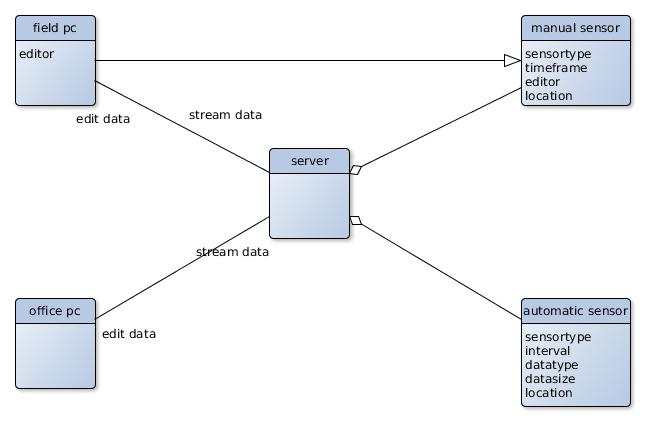
\includegraphics[scale=0.6]{graphics/model_of_issue.jpg} 
	\caption{Modell des Problembereiches mit relevanten Objekten, F. H. Euteneuer 2013}
	 \label{fig:model_domain}
\end{figure}

Die Datenbank die and den \gls{Server} angeschlossen ist speichert sowohl Metadaten zu den Sensoren, als auch die gemessenen Werte. Unter Metadaten sind alle Informationen zu verstehen, die die Sensoren eindeutig beschreiben, und die für weitere Analysen der Messerwerte erforderlich sind (siehe auch im Glossar "Metadaten". Beispielsweise sind das die Positionen der Sensoren, die Messintervalle, die Sensortypen oder die übermittelten Datentypen.

Als Klient des Services kann im Prinzip jede Art von mobilen Systemen eingesetzt werden. Angeschlossen an die Datenbank dienen diese dann als bildgebender Teil des Systems. Da die Verknüpfung mit einem \gls{Server} meist über das Protokoll \newacronym{TCP/IP}{TCP/IP}{Transmission Control Protocol/Internet Protocol} \gls{TCP/IP} geschieht, müssen mobile Geräte über eine Internetverbindung verfügen. Die Verwendung dieser Geräte bleibt dadurch begrenzt auf Gebiete innerhalb der Handynetz-Abdeckung. Für manuelle Messungen dient der mobile Klient zusätzlich als Eingabegerät für die Messwerte, sofern dies nicht über das Gerät selber erfolgen kann. Dadurch wird der mobile Klient in dem Modell sowohl als bildgebender Teil des Systems, als auch als Sensor behandelt, und ererbt damit die Eigenschaften des Sensor Objekts.

Das System will einen ganzheitlichen Ansatz verfolgen, und beinhaltet somit auch einen Teil der für die umfangreicheren Analysen zuständig ist, sowie durch eine Datenexportfunktion als Schnittstelle zu weiteren Algorithmen und System dient. Dieser Teil des System wird in dem Modell durch den "Desktop-Computer" repräsentiert. Die eigentliche Einrichtung und Planung des Systems wird erwartungsgemäß von diesem, dem bequemeren Arbeitsplatz (verglichen mit dem mobilen Klienten), durchgeführt werden. Zusätzlich zu den Eigenschaften des Feldcomputers sind somit erweiterte Verwaltungs- und Analysefunktionen als Eigenschaften dieses Objektes definiert.


\subsection{Geschäftsprozesse}
Wichtigste Entscheidungshilfe für die Nutzung solch eines Systems wird die Eigenschaft des Systems, eine entscheidungsunterstützende Funktion zu erfüllen, sein. Das System ist fokussiert auf die wichtigen Werkzeuge die die Arbeit des Feldingenieurs vereinfachen sollen, und lässt unwichtige oder komplizierte Werkzeuge komplett weg. Außerdem werden die Informationen die im Feld auf dem mobilen Klienten angezeigt werden derart reduziert, dass lediglich aussagekräftige Werte, die damit Entscheidungen unterstützen können, angezeigt werden. In dem vorherigem Kapitel habe ich den Problembereich beschrieben, nun möchte ich die verschiedenen Prozesse skizzieren die ein Nutzer durchführen könnte.

\begin{figure}[H]
	\centering
 	 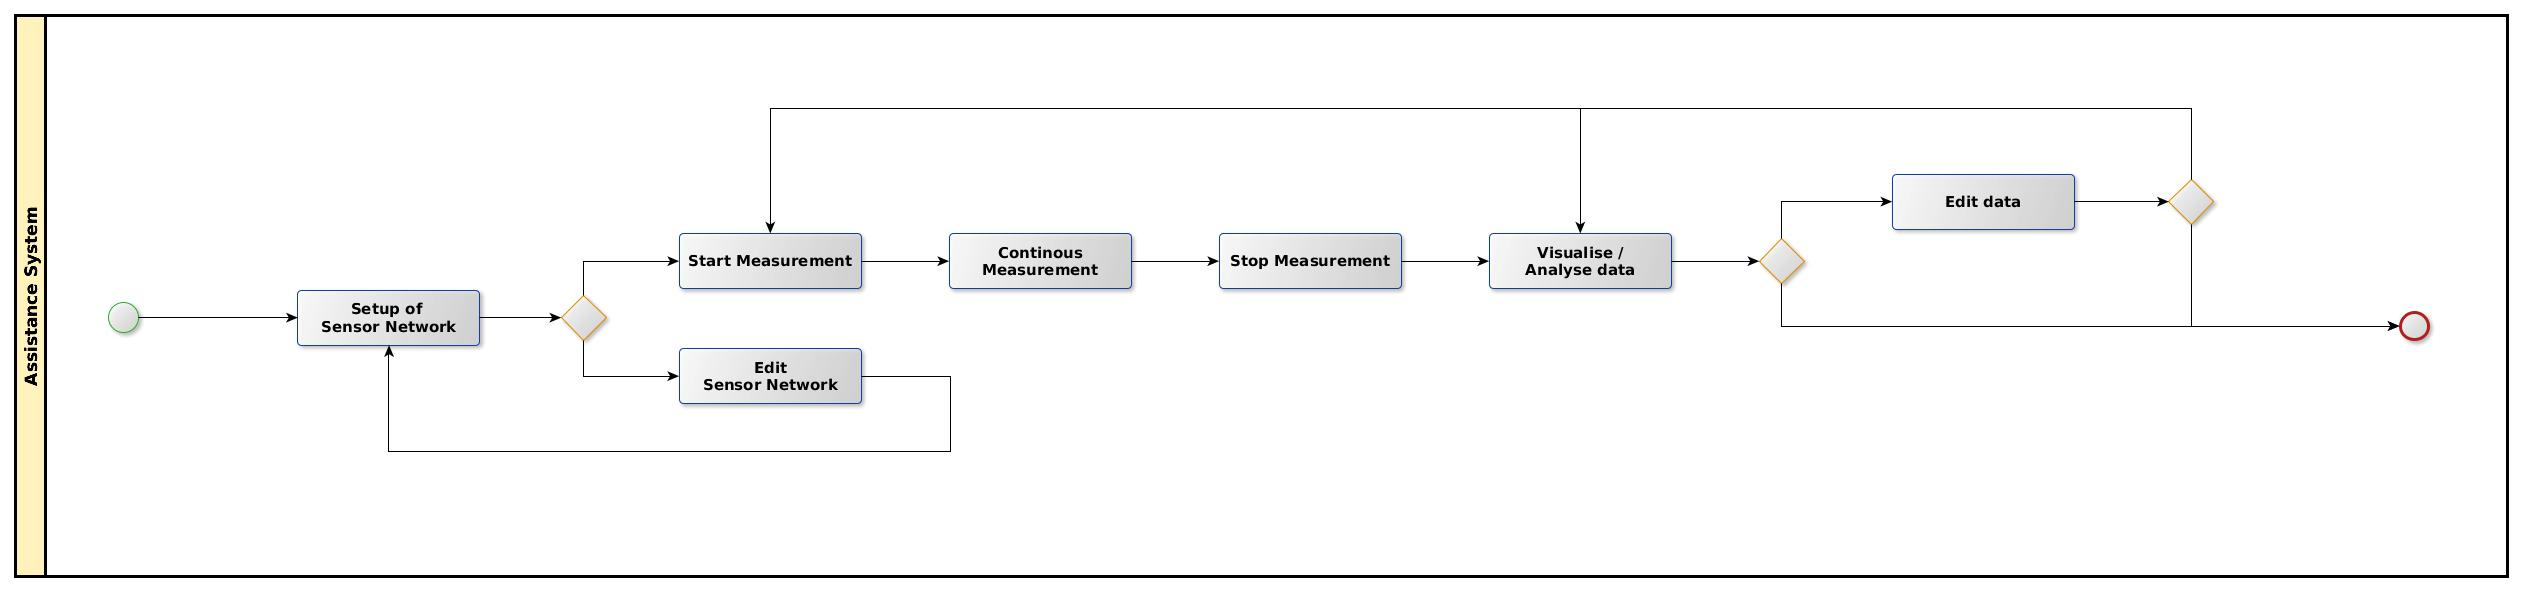
\includegraphics[scale=0.2]{graphics/bpmn_business-processes.jpg} 
	\caption{BPMN (Business Process Model and Notation) Modell relevanter Aktionen welche in dem System durchgeführt werden, F. H. Euteneuer 2013}
	 \label{fig:model_business-processes}
\end{figure}

Ich habe drei verschiedene Hauptaktionen identifiziert, die ein Nutzer durchführen könnte: Das manuelle Messen von Werten, das manuelle Editieren bereits gemessener Werte, und das automatische kontinuierliche Messen. Die Abbildung \ref{fig:model_business-processes} veranschaulicht mittels eines \gls{UML} Activity Diagrams (\gls{UML} Aktivitäten Diagramm) die einzelnen Abläufe dieser Aktionen.

Die manuelle Messung beginnt mir der normalen Messung der Werte. Im zweiten Schritt erfolgt die Eingabe der Werte in das System. Die Werte werden automatisch auf ihre Validität hin überprüft, und erste einfache statistische Analysen werden erstellt. Diese erste Statistik ist erforderlich um Informationen über die Qualität der Messung zu erhalten, und dem System die Möglichkeit zu bieten fehlerhafte Messungen zu bemängeln und Neumessungen vorzuschlagen.

Der Nutzer wird die Möglichkeit haben vergangene Messungen manuell zu bearbeiten. Dazu muss ein Datensatz (Üblicherweise ein Messwert) ausgewählt werden, und der Nutzer kann dann entscheiden ob die betreffende Messung wiederholt werden soll, oder die Werte manuell geändert werden sollen. Bei einer Wiederholung der Messung wird die Prozesskette der manuellen Messung durchlaufen.

Die automatische Messung ist die wichtigste Funktion des Systems, und stellt eine der Innovationen dar. Obwohl das Verfahren ein anderes ist, sind die zu Grunde liegenden Funktionen der manuellen und der automatischen Messung sehr ähnlich. Als initiale Handlug muss das Sensor Netzwerk eingerichtet werden, dazu gehören die Eingabe der Metadaten, wie Sensor-Typ und -Position oder benutztes geographisches Referenz System. Welche Parameter tatsächlich benötigt werden um ein lauffähiges Sensoren Netzwerk einzurichten, wird in später folgenden methodischen Teilen genauer beschrieben. Nach der Einrichtung des Netzwerkes hat der Nutzer die Möglichkeit kontinuierliche automatische Messungen zu starten, und später auch wieder zu stoppen. Auch ein nachträgliches Ändern der eingegebenen Parameter ist möglich.

Zum Abschluss dieses Kapitels möchte ich nochmal darauf hinweisen, dass die hier beschriebene Liste an Funktionalitäten lediglich ein sehr rudimentäres System beschreiben, und demnach auch keinen Anspruch auf Vollständigkeit erhebt.


\section{Produktfunktionen}
Was muss das System nun an Funktionalität anbieten, um den genannten Ansprüchen gerecht zu werden? Um diese Frage besser beantworten zu können möchte ich einige Anwendungsfälle beschreiben, in denen verschiedene Nutzergruppen für sie interessante Aufgaben mit Hilfe des System lösen werden. Nach einer kurzen Beschreibung der verschiedenen Nutzergruppen werde ich jeden Anwendungsfall in tabellarischer Form analysieren.

\begin{figure}[H]
	\centering
 	 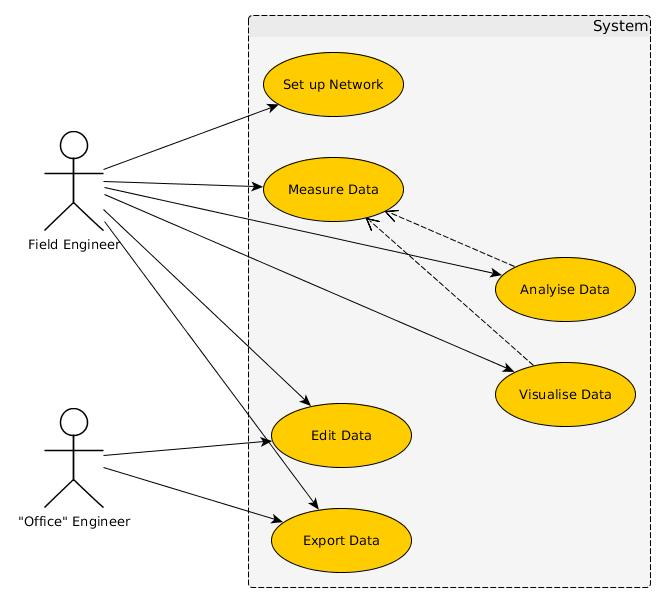
\includegraphics[scale=0.6]{graphics/uml_functionalities.jpg} 
	\caption{UML Anwendungsfalldiagram des beschriebenen Systems und der einzelnen Nutzergruppen mit ihren Anwendungsfällen, F. H. Euteneuer 2013}
	 \label{fig:model_functionalities}
\end{figure}

\subsection{Nutzergruppen}
Die Analyse der verschiedenen Nutzergruppen des Systems bildet eine wichtige Informationsquelle für die Konzeption des Systems. Anstatt wahllos Funktionen zu beschreiben, die vermutlich in ein System gehören sollten, werden so imaginäre aber präzise definierte Nutzer identifiziert und befragt, was sie mit diesem System anfangen wollen. Die Abbildung \ref{fig:model_functionalities} enthält bereits die zwei identifizierten wichtigsten Nutzergruppen die in die Prozesse involviert sind.

\subsubsection{Feldingenieure}
Die Gruppe der Feldingenieure kann als die Gruppe der Ausführenden Personen beschreiben werden, die im direkten Kontakt zu den Sensoren stehen oder selbst manuell die Messungen durchführen. Für die Kommunikation mit dem System verwenden sie einen mobilen Klienten, dadurch sind sie technisch bestimmten Restriktionen unterworfen. In der Folgenden Liste sind die wichtigsten benannt:
\begin{itemize}
\item Kleine Anzeigefläche auf dem Mobilen Klienten (Qualität der Visualisierung ist limitiert)
\item Fehlende oder mangelhafte Eingabemöglichkeiten (z.B.: Eingabe nur durch virtuelle Tastatur auf einem Mobilen Computer)
\item Hohes Gewicht von nicht mobilen Klienten (z.B.: Verwendung eines konventionellen Notebooks als mobile Lösung, für Arbeiten im stehen oder Laufen aber zu schwer)
\end{itemize}
Nichtsdestotrotz definiert diese Nutzergruppe die herausfordernsten Anforderungen an das System, beispielsweise durch die Implementierung einer intelligenten Visualisierungsmöglichkeit. Da diese Nutzergruppe die eigentliche Zielgruppe des Systems darstellt, sollten die Anforderungen dieser Gruppe zu gut als möglich erfüllt werden.

\subsubsection{Bürokraft}
Normalerweise sind die Nutzer Feld- und Büroingenieur vereinigt in einer Person. Projekte die sich mit der Überwachung von Bauwerken befassen können in zwei Teile untergliedert werden. Ein Teil ist für die Installation des Netzwerkes, für etwaige manuelle Messungen und für die Betreuung bestehender Sensornetzwerke zuständig, während sich der andere Teil um die Auswertung der eingehenden Daten, die "Postprozessierung" (DE: Nachbearbeitung) und die Interpretation der Daten kümmert. Durch die meist sehr komfortabel ausgestattete Informationstechnologie in den Büros erwarte ich hier niedrigere technische Anforderungen an das System.

\subsection{Anwendungsfälle}
Die Abbildung \ref{fig:model_functionalities} zeigt die grundlegenden unterschiedlichen Anwendungsfälle der zwei im vorherigen Kapitel beschriebenen Nutzergruppen. Anwendungsfälle die in der Abbildung genannt werden repräsentieren Handlungsfolgen des jeweiligen Nutzers, die innerhalb des Anwendungsfalles abgeschlossen sein müssen, also ein festgelegtes Ziel erreichen müssen. Ich werde nun die Anwendungsfälle wie bereits erwähnt in tabellarischer Form mit weiteren Parametern beschreiben. Dieser Arbeitsschritt ist essentiell für Planung und Konzeption eines Systems, da hierdurch der tatsächliche Bedarf der Nutzer und damit die zu implementierenden Funktionalitäten beschrieben werden.

Ich werde alle Anwendungsfälle zunächst mit einem Text einleiten, und dann in der Tabelle die wichtigsten Eigenschaften beschreiben. Dazu gehören das festgelegte Ziel eines Anwendungsfalles oder die sogenannte Nachbedingung, die beschreibt in welcher Situation sich das System nach dem erfolgreichem Durchlaufen eines Anwendungsfalles befindet. Anschließend werden die einzelnen zu durchlaufenden Schritte der Anwendungsfälle in einem \gls{UML} Aktivitäten Diagramm veranschaulicht.

Ich habe die verschiedenen Anwendungsfälle in drei Gruppen gegliedert. Jeweils zwei Anwendungsfälle decken die Gebiete des Daten Managements, der Daten Analyse und der eigentlichen Messung ab.

Die hier vorgestellten Anwendungsfälle repräsentieren keinesfalls alle Arbeitsabläufe die möglich sind, sondern sollen nur einen möglichen Lösungsweg beschreiben, der in dem Prototyp implementiert werden könnte.

\subsubsection{Management}
Management soll hier sowohl für das Management von Daten als auch für das Einrichten und die Betreuung des Systems stehen. Erster Anwendungsfall soll das Aufsetzen eines Sensornetzwerkes beschreiben. Das kann auch als initiale Handlung bei der Verwendung des Systems gesehen werden, und ist damit eine Art Vorbedingung für alle nachfolgenden Anwendungsfälle. Die Tabelle \ref{table:use case description of "Set up network"} beinhaltet die zentralen Eigenschaften dieses Anwendungsfalles.

Das Datenmanagement ist ein erforderlicher Teil eines Systems das sich mit Daten und Metadaten befasst. Daten zu sammeln ohne sie nutzen zu können würde keinen Sinn ergeben, somit ist ein Export der Daten aus dem System heraus eine obligatorische Funktion des Systems. Dieser Anwendungsfall kann also auch als finale Handlung gesehen werden, die unter Verwendung des Systems durchgeführt werden wird. Die zweite Tabelle \ref{table:use case description of "Export data"} beinhaltet detailierte Informationen über diesen "Datenexport" genannten Anwendungsfall.

\begin{table}[H]
\centering
\begin{tabular}{l | p{11cm}}
Name & Einrichtung des Netzwerkes\\ \hline 
Nutzergruppe & Feldingenieur\\ \hline 
Ziel & Eingabe aller Metadaten über die verbundenen Sensoren und Initialisierung des Netzwerkes\\ \hline 
Vorbedingung & Das Netzwerk existiert, ist eingerichtet und ist mit dem System verbunden\\ \hline 
Nachbedingung & Funktionierendes Netzwerk mit allen Sensoren\\ 
\end{tabular}
\caption{Tabellarisierte Beschreibung aller Charakteristika des Anwendungsfalls "Einrichtung des Netzwerkes"} 
\label{table:use case description of "Set up network"}
\end{table}

\begin{table}[H]
\centering
\begin{tabular}{l | p{11cm}}
Name & Datenexport\\ \hline 
Nutzergruppe & Bürokraft\\ \hline 
Ziel & Auswahl der Daten und Export in einem bestimmten Format\\ \hline 
Vorbedingung & Auswahl der Daten nach bestimmten Parametern und spezifiziertes Exportformat\\ \hline 
Nachbedingung & Ausgewählte Daten liegen vollständig physikalisch im definiertem Format vor\\ 
\end{tabular}
\caption{Tabellarisierte Beschreibung aller Charakteristika des Anwendungsfa'
lls "Datenexport"}\label{table:use case description of "Export data"}
\end{table}

Die Abbildung \ref{fig:bpmn_use-case_management} zeigt die Anwendungsfälle die sich mit der Thematik des Managements befassen in einem \gls{UML} Aktivitätsdiagramm. Die beiden Abläufe weisen keine Interaktionen untereinander auf und sind damit vollständig unabhängig voneinander. Chronologisch hingegen sollte das Einrichten des Netzwerkes vor dem Datenexport erfolgen.

Der Ablauf des Einrichtens des Netzwerkes beinhaltet zwei wichtige Aktionen: Zum Einen das Einrichten der Datenbank und zum Anderen die Eingabe der Sensorparameter. Dies sind die zwei zentralen teile dieses Anwendungsfalls, und ein scheitern nur eines dieser Aktionen würde zu einem nicht funktionierendem Netzwerk führen. Die Bearbeitung der "Netzwerkeinstellungen", also der einzelnen eingegebenen Parameter, führt zu einem erneutem Durchlaufen der gesamten Prozesskette. Damit sollen fehlerhafte Eingaben vermieden werden, diese Funktion stellt eine Art Assistenzsystem dar, das durch alle wichtigen Einstellmöglichkeiten führt.

Der Anwendungsfall "Datenexport" ist um Einiges einfacher als der vorherige, im Prinzip ähnelt er den meisten klassischen Exportfunktionen oder Speicherfunktionen. Einzig die Auswahl der zu exportierenden Daten durch das setzen eines Zeitrahmens stellt eine größere Herausforderung an das System dar.

\begin{figure}[H]
	\centering
 	 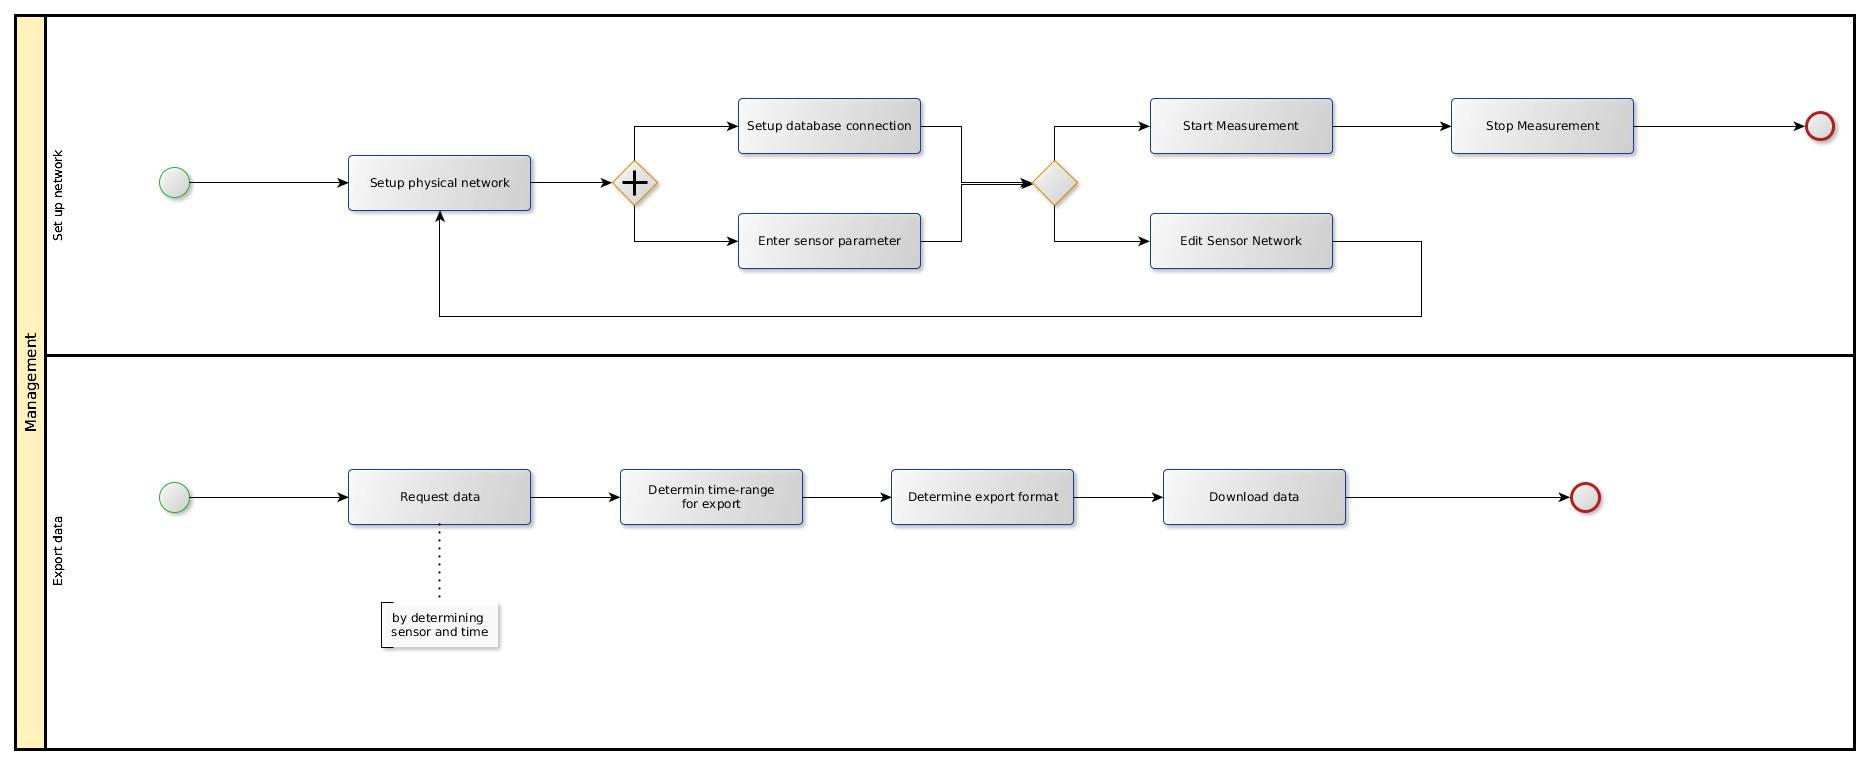
\includegraphics[scale=0.24]{graphics/bpmn_use-cases_management.jpg} 
	\caption{BPMN (Business Process Model and Notation) Modell der Management Anwendungsfälle, F. H. Euteneuer 2013}
	 \label{fig:bpmn_use-case_management}
\end{figure}


\subsubsection{Messungen}
Der Teil des Systems der sich mit den eigentlichen Messungen beschäftigt, könnte als der wichtigste Teil gesehen werden, stellt aber an sich keine wesentliche Innovation dar. Dieser Teil beschreibt als Einziger die manuelle Bearbeitung oder Veränderung der Daten in der Datenbank.

In diesem Teil habe ich zwei wichtige Anwendungsfälle identifiziert: Der Erste beschäftigt sich mit dem initialen "Dateninput", also der Eingabe von Daten, produziert durch Messungen. Die Charakteristiken dieses Anwendungsfalles sind in der Tabelle \ref{table:use case description of "Measure data"} beschrieben. Im Gegensatz zu den automatischen Messungen beschreibt dieser Anwendungsfall die manuelle Eingabe von nur einem Datensatz.

Der Zweite Anwendungsfall behandelt das manuelle Bearbeiten der bereits in der Datenbank gespeicherten Werte. Die Tabelle \ref{table:use case description of "Edit data"} beinhaltet alle wichtigen Informationen dazu. Das Bearbeiten von Daten gehört zu den Standardoperationen für System die sich auf Datenbanken stützen. Dennoch ist es wichtig zu beschreiben, wie dieser Anwendungsfall mit dem der Messungen zusammenhängt. Im Falle von Neumessungen bestimmter Werte oder des Validieren von Daten wird die Prozesskette der Messung durchlaufen obwohl es im Grunde eine Bearbeitung bereits bestehender Werte ist.

\begin{table}[H]
\centering
\begin{tabular}{l | p{11cm}}
Name & Messung\\ \hline 
Nutzergruppe & Feldingenieur\\ \hline 
Ziel & Eingabe aller Messergebnisse von Einzelmessungen per Hand\\ \hline 
Vorbedingung & Lauffähiges System mit Verbindung zur Datenbank\\ \hline 
Nachbedingung & Gültige Daten in der Datenbank mit vollständigen Metadaten\\ 
\end{tabular}
\caption{Tabellarisierte Beschreibung aller Charakteristika des Anwendungsfalls "Messung"} 
\label{table:use case description of "Measure data"}
\end{table}

\begin{table}[H]
\centering
\begin{tabular}{l | p{11cm}}
Name & Datenbearbeitung\\ \hline 
Nutzergruppe & Bürokraft\\ \hline 
Ziel & Auswahl der Datensätze nach Parametern und Bearbeitung der Werte per Hand oder durch Neumessung\\ \hline 
Vorbedingung & Lauffähiges System mit Verbindung zur Datenbank\\ \hline 
Nachbedingung & Veränderte Daten in der Datenbank mit vollständigen Metadaten\\ 
\end{tabular}
\caption{Tabellarisierte Beschreibung aller Charakteristika des Anwendungsfalls "Datenbearbeitung"} 
\label{table:use case description of "Edit data"}
\end{table}

Bei manuellen Messungen sind die Aktionen die in der oberen Reihe des Aktivitätendiagrammes \ref{fig:bpmn_use-case_measuring} angegeben werden unabdingbar. Das System wird nach der Durchführung der Messungen eine schnelle Analyse der Messergebnisse durchführen um deren Qualität zu bewerten. Nach diesem Schritt wird das System entweder auf mögliche Fehler in der Messung hinweisen, oder die Messwerte direkt in die Datenbank schreiben. 

Die zweite Linie des Diagramms beschreibt die Handlungskette der Datenbearbeitung. Der Nutzer hat zwei Möglichkeiten Daten nachträglich zu bearbeiten, zum Einen durch die erneute Messung der Daten, zum Anderen durch das manuelle Bearbeiten, also die Eingabe neuer Werte und das Überschreiben der alten Werte. 

\begin{figure}[H]
	\centering
 	 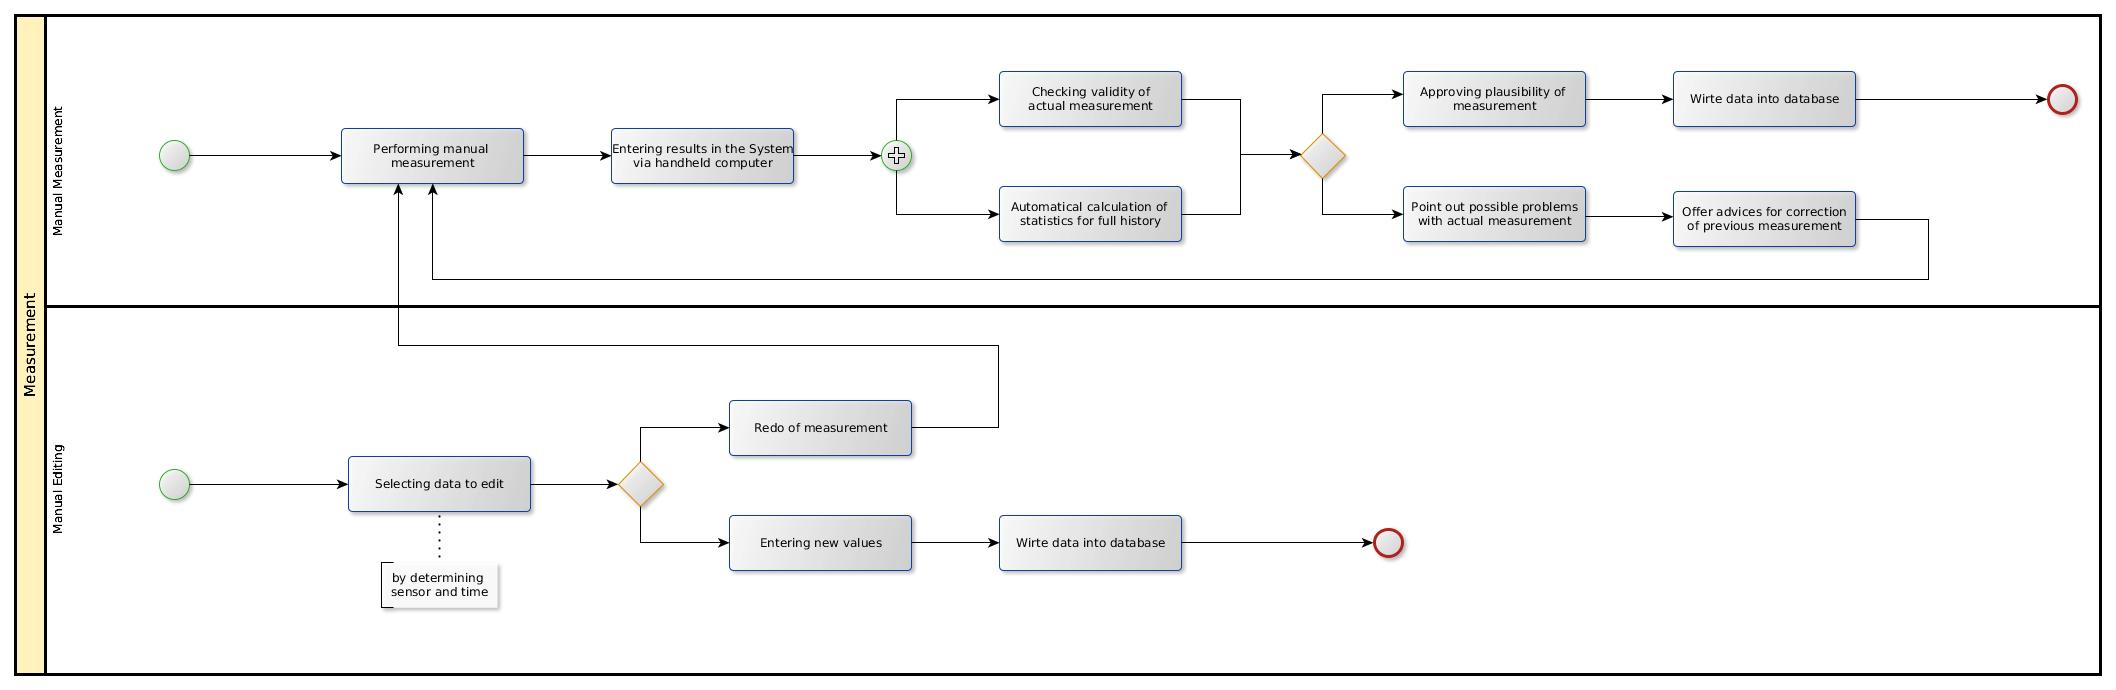
\includegraphics[scale=0.24]{graphics/bpmn_use-cases_measurement.jpg} 
	\caption{BPMN (Business Process Model and Notation) Modell der Anwendungsfälle des Teiles Messungen, F. H. Euteneuer 2013}
	 \label{fig:bpmn_use-case_measuring}
\end{figure}

\subsubsection{Analyse}
In den vorherigen Kapiteln habe ich oft von einer Analyse der Daten gesprochen, bislang aber nichts Genaueres dazu gesagt. Die Analyse stellt den wohl schwierigsten Teil der Konzeption dar, weil dieser die eigentliche Innovation darstellt. Die Analyse die ich hier beschreiben werde unterscheidet sich allerdings von der auch oft erwähnten Überprüfungen der Daten. Diese "ad hoc" Statistiken stellen lediglich eine schnelle und unpräzise Vorabinformation über die Qualität der Daten dar. Um die Frage beantworten zu können ob Messungen einen Sinn ergeben, also die Konsistenz der Daten beurteilen zu können, bedarf es komplexere Algorithmen, die außer den eigentlich zu beurteilenden Daten auch die vorhergegangenen Beobachtungen (Epochen) mit einbeziehen. Diese Algorithmen erzeugen trotzdem nur eine schnelle Übersicht über Mögliche Abweichungen oder Ereignisse, nichtsdestotrotz wird der Nutzer mithilfe dieser Analysen in der Lage sein Mögliche Verfahrensfehler bei den Messungen direkt im Feld zu identifizieren. Die Funktionalität wird in der tabellarischen Beschreibung \ref{table:use case description of "Analyse data"} des Anwendungsfalls "Datenanalyse" charakterisiert.

Der zweite Teil des Analyse Bereiches basiert auf einer visuellen Analyse der Daten durch den Nutzer. Kern dieser Funktionalität sind eine Visualisierung des zu überwachenden Objektes und der Ergebnisse bereits erfolgter Analysen und werden in der Tabelle \ref{table:use case description "Visualise data"} charakterisiert. Das System wird eine grafisches Modell des zu überwachenden Objektes generieren, und die Optionen anbieten Messergebnisse und berechnete Statistiken ebenfalls in die Grafik zu integrieren. Der Nutzer ist dann in der Lage Messungen in Echtzeit zu überwachen, und beispielsweise auch Auswirkungen von Experimenten zu verfolgen. Die Art und Weise der Visualisierung von Objekt, Messung und Statistik wird genauer im methodischen Teil der Arbeit beschrieben.

\begin{table}[H]
\centering
\begin{tabular}{l | p{11cm}}
Name & Datenvisualisierung\\ \hline 
Nutzergruppe & Feldingenieur\\ \hline 
Ziel & Visuelle Unterstützung bei Messungen und Interpretation\\ \hline 
Vorbedingung & Vorhandene Metadaten für die Betreffende Messung (z.B. verwendeter Sensor, Orientierung, ..)\\ \hline 
Nachbedingung & Aussagekräftige und "unterstützende" Grafik der ausgewählten Daten\\
\end{tabular}
\caption{Tabellarisierte Beschreibung aller Charakteristika des Anwendungsfalls "Datenvisualisierung"} 
\label{table:use case description "Visualise data"}
\end{table}

\begin{table}[H]
\centering
\begin{tabular}{l | p{11cm}}
Name & Datenanalyse\\ \hline 
Nutzergruppe & Feldingenieur\\ \hline 
Ziel & Erhalt von Informationen über Gültigkeit der Daten verglichen mit vergangenen Epochen\\ \hline 
Vorbedingung & Bereits mehr als zwei Messungen liegen vor\\ \hline 
Nachbedingung & Informationen über Gültigkeit der Messergebnisse\\ 
\end{tabular}
\caption{Tabellarisierte Beschreibung aller Charakteristika des Anwendungsfalls "Datenanalyse\\"} 
\label{table:use case description of "Analyse data"}
\end{table}

Die Abbildung \ref{fig:bpmn_use-case_analysis} zeigt die Ereignisabläufe der beiden ausgewählten und beschriebenen Anwendungsfälle des Analyseteils des Systems. In der ersten Reihe ist als wichtiger Schritt die Definition der historischen Daten hervorzuheben. Erst damit werden Werte aussagekräftig.

Die Visualisierung der Daten ins untergliedert in zwei Typen. Der Nutzer kann zwischen der Visualisierung der gemessenen Werte und der berechneten Statistiken wählen. Für die Visualisierung der Statistiken müssen die Statistiken bereits berechnet worden sein. Die Durchführung der Analyse kann auch aus der Visualisierungsfunktion heraus aufgerufen werden.

\begin{figure}[H]
	\centering
 	 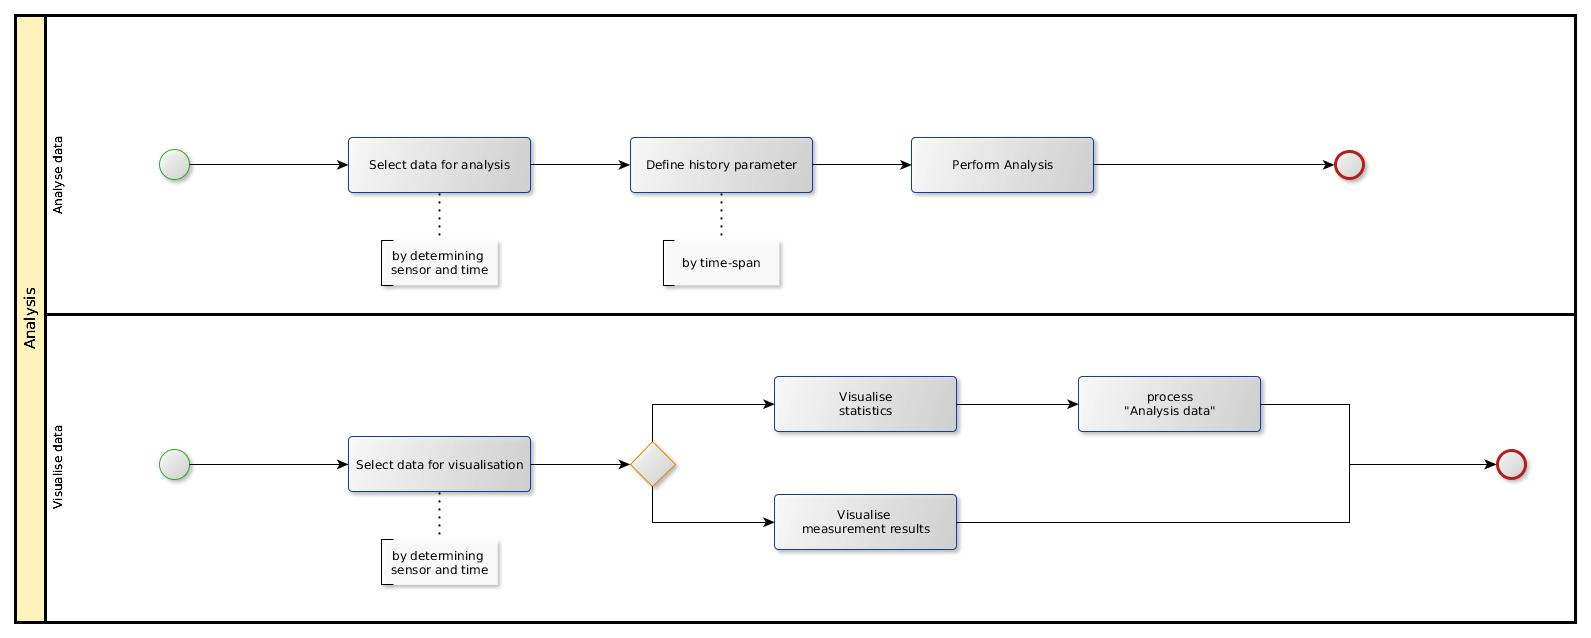
\includegraphics[scale=0.24]{graphics/bpmn_use-cases_analysis.jpg} 
	\caption{BPMN (Business Process Model and Notation) Modell der Anwendungsfälle des Teiles Analyse, F. H. Euteneuer 2013}
	 \label{fig:bpmn_use-case_analysis}
\end{figure}


\section{Produktfunktionen}
In diesem Kapitel beschreibe ich die nicht-funktionalen Anforderungen an das System beschreiben. Nicht-funktional bedeutet, dass beschrieben wird wie das System wo eingesetzt werden soll. Es handelt sich also um Eigenschaften des Systems, die keine technischen Funktionen sind.

Im Folgenden werden die nicht-funktionalen Anforderungen aufgelistet und beschrieben:
\begin{description}
\item[Portabilität] Da das System besonders auf die Kommunikation zwischen der Arbeit im Feld und der Auswertung im Büro zugeschnitten ist, werden besondere Anforderungen an die Möglichkeit der Portierung auf verschiedene Betriebssysteme der mobilen Klienten gestellt. Das System soll damit Plattform-unabhängig sein. 
\item[Rechenleistung] Wie im Punkt zuvor beschrieben soll das System auf unterschiedlichen mobilen Klienten eingesetzt werden können. Deren Auslegung auf die Mobilität geht meist zu Lasten der Rechenleistung der Hardware. Damit das Arbeiten mit dem System dennoch effizient und einfach gehalten werden kann, muss der mobile Teil des Systems für diese kleine Rechenleistung zugeschnitten werden.
\item[Einfachheit] Die Hauptnutzer des Systems werden Ingenieure sein, die oft unter schwierigen Bedingungen arbeiten müssen. Die Bedienung eines IT-Systems sollte demnach so intuitiv und einfach wie möglich gestaltet werden, damit der Nutzer nicht unnötig Zeit in die Suche von Funktionen oder das Verstehen von Grafiken aufbringen muss.
\end{description}




